\section{The Fast Fourier Transform}

We begin this review by looking at the waveform shown in Figure \ref{fig:FFT Sample Waveform}.
When we take the Fast Fourier Transform (FFT) of this signal, we get an output that is complex and exactly the same length.
Since the FFT algorithm doesn't know what our sampling frequency is, we must create our own frequency array. We do so by creating a linear array of numbers between zero and one that is equal in length to the length of the original waveform (which is equal in length to the FFT output).
We then multiply this array by the sampling frequency so that our results range between zero and out sampling frequency.
This calculation is shown in Equation \ref{eq:Create Frequency Array For FFT}.

\begin{equation} \label{eq:Create Frequency Array For FFT}
    f = \text{fs * linspace(0,1,length(waveform))}
\end{equation}

where

\begin{itemize}
    \item fs = sampling frequency
    \item linspace = a common command in many programming languages, used to create a linear array between two numbers
    \item waveform = the original waveform
\end{itemize}

\begin{figure}[H]
    \centering
    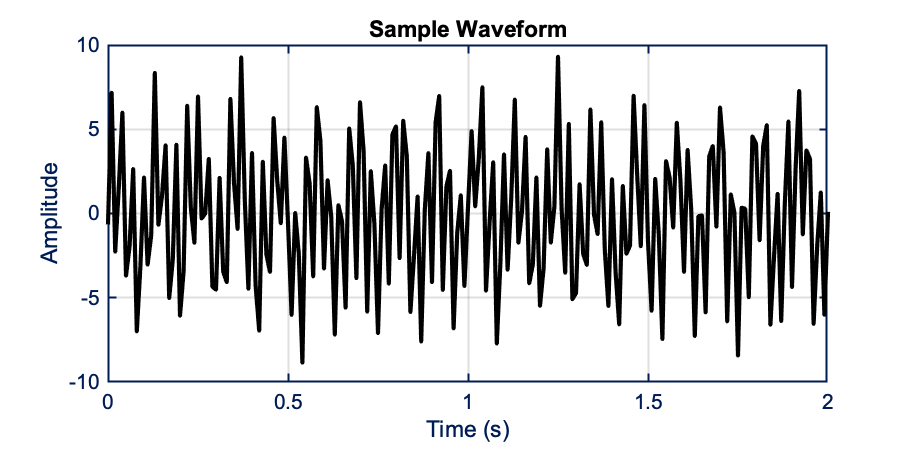
\includegraphics[width = 6 in]{Chapters/Signal Processing/Figures/Sample Waveform.png}
    \caption{A sample waveform for use in the FFT review. I have placed tones at 9 and 33 Hz along with gaussian-distributed random noise. The sampling frequency is 100 Hz.}
    \label{fig:FFT Sample Waveform}
\end{figure}

Once this frequency array is created, we can start looking at the output.
For a real-valued input signal, we will get a complex result.
The raw FFT for the waveform shown in Figure \ref{fig:FFT Sample Waveform} is shown in Figure \ref{fig:Raw FFT Output}.
The real part describes the amplitude of the frequencies, and the imaginary part describes the phase.

\begin{figure}[H]
    \centering
    \includegraphics[width = 6 in]{Chapters/Signal Processing/Figures/Raw FFT Output.png
    \caption{The raw output of the FFT function in MATLAB, showing both the real (left) and imaginary (right) parts of the output.}
    \label{fig:Raw FFT Output}
\end{figure}